
This section is devoted to the development of all the notions and results necessary to understand and prove the spectral theorem, stated below. 

\bt[Spectral theorem]
\label{thm:Spectral}
For every self-adjoint operator $A\cl \mathcal{D}_A\to \mathcal{H}$ there is a unique projection-valued measure $\mathrm{P}_{\negmedspace A}\cl \sigma(\mathcal{O}_{\R})\to\mathcal{L}(\mathcal{H})$ such that
\bse
A = \int_{\R}\! i_{\R} \, \d \mathrm{P}_{\negmedspace A} \equiv \int_{\R}\! \lambda \, \mathrm{P}_{\negmedspace A}(\d \lambda),
\ese
where $i_{\R}\cl \R\hookrightarrow \C$ is the inclusion of $\R$ into $\C$.
\et

While useful in theory, existence results are often of limited use in practice since they usually only tell us that something exists, and not how to construct it. However, we should note here that the proof of the spectral theorem is, in fact, constructive in nature. Hence, given any self-adjoint operator $A$, we will be able to explicitly determine its associated projection-valued measure $\mathrm{P}_{\negmedspace A}$ along the following steps.
\begin{enumerate}[label=(\roman*)]
\item For each $\psi\in\mathcal{H}$, construct the real-valued Borel measure $\mu^A_{\psi}\cl \sigma(\mathcal{O}_{\R})\to \R$ given by
\bse
\mu^A_{\psi} ((-\infty,\lambda]):= \lim_{\delta\to 0^+} \lim_{\varepsilon\to 0^+} \int_{-\infty}^{\lambda+\delta}\!\d t  \Im\langle\psi | R_A(t+\mathrm{i}\varepsilon)\psi\rangle ,
\ese
where $R_A\cl\rho(A)\to \mathcal{L}(\mathcal{H})$ is the resolvent map of $A$. This is know as the \emph{Stieltjes inversion formula}. Note that while not every element in $\sigma(\mathcal{O}_{\R})$ is of the form $(-\infty,\lambda]$, such Borel measurable sets do generate the entire $\sigma(\mathcal{O}_{\R})$ via unions, intersections and set differences. Hence, the value of $\mu^A_{\psi}(\Omega)$ for $\Omega\in\sigma(\mathcal{O}_{\R})$ can be determined by applying the corresponding formulae for measures, namely $\sigma$-additivity, continuity from above and measure of set differences.
\item For all $\psi,\varphi\in\mathcal{H}$, define the complex-valued Borel measure $\mu^A_{\psi,\varphi}\cl\sigma(\mathcal{O}_{\R})\to\C$ by
\bse
\mu^A_{\psi,\varphi}(\Omega):=\tfrac{1}{4}(\mu^A_{\psi+\varphi}(\Omega)-\mu^A_{\psi-\varphi}(\Omega)+\mathrm{i}\mu^A_{\psi-\mathrm{i}\varphi}(\Omega)-\mathrm{i}\mu^A_{\psi+\mathrm{i}\varphi}(\Omega)).
\ese
\item Define the projection-valued measure $\mathrm{P}_{\negmedspace A}\cl \sigma(\mathcal{O}_{\R})\to\mathcal{L}(\mathcal{H})$ by requiring $\mathrm{P}_{\negmedspace A}(\Omega)$, for each $\Omega\in\sigma(\mathcal{O}_{\R})$, to be the unique map in $\mathcal{L}(\mathcal{H})$ satisfying
\bse
\forall\, \psi,\varphi\in\mathcal{H}:\ \langle\psi|\mathrm{P}_{\negmedspace A}(\Omega)\varphi\rangle = \int_{\R}\!\chi_{\Omega}\,\d\mu^A_{\psi,\varphi}.
\ese
\end{enumerate}

We will now make all the notions and constructions used herein precise. In fact, we will present the relevant definitions and results by taking the inverse route, starting with projection-valued measures and arriving at their associated self-adjoint operators, obtaining (and proving) what we will call the inverse spectral theorem.

\subsection{Projection-valued measures}

Projection-valued measures are, unsurprisingly, objects sharing characteristics of both measures and projection operators.

\bd
A map $\mathrm{P}\cl \sigma(\mathcal{O}_{\R})\to\mathcal{L}(\mathcal{H})$ is called a \emph{projection-valued measure}\index{projection-valued measure} if it satisfies the following properties.
\ben[label=(\roman*)]
\item $\forall\, \Omega \in \sigma(\mathcal{O}_{\R}) : \ \mathrm{P}(\Omega)^* = \mathrm{P}(\Omega) $
\item $\forall\, \Omega \in \sigma(\mathcal{O}_{\R}) : \ \mathrm{P}(\Omega)\circ \mathrm{P}(\Omega) = \mathrm{P}(\Omega) $
\item $\mathrm{P}(\R)=\id_{\mathcal{H}}$
\item For any pairwise disjoint sequence $\{\Omega_n\}_{n\in\N}$ in $\sigma(\mathcal{O}_{\R})$ and any $\psi\in\mathcal{H}$,
\bse
\sum_{n=0}^{\infty}\mathrm{P}(\Omega_n)\psi = \mathrm{P}\biggl(\bigcup_{\, n=0}^{\infty}\Omega_n\biggr)\psi.
\ese
\een
\ed

\br 
Note in the final condition we included $\psi\in\cH$ as, for the case countably infinite $n\in\N$ we need to check convergence, which involves using the norm. Without the $\psi$ we would need to use the norm on $\cL(\cH)$ which may prove difficult. However, by including the $\psi$ we can work with the norm on $\cH$ itself. 
\er 

\bl
Let $\mathrm{P}\cl \sigma(\mathcal{O}_{\R})\to\mathcal{L}(\mathcal{H})$ be a projection-valued measure. Then, for any $\Omega,\Omega_1,\Omega_2\in\sigma(\mathcal{O}_{\R})$,
\ben[label=(\roman*)]
\item $\mathrm{P}(\varnothing)=0$, where by $0$ we mean $0\in\mathcal{L}(\mathcal{H})$
\item $\mathrm{P}(\R\setminus \Omega)={\id_{\mathcal{H}}}-\mathrm{P}(\Omega)$
\item $\mathrm{P}(\Omega_1\cup\Omega_2)=\mathrm{P}(\Omega_1)+\mathrm{P}(\Omega_2)-\mathrm{P}(\Omega_1\cap\Omega_2)$
\item $\mathrm{P}(\Omega_1\cap\Omega_2)=\mathrm{P}(\Omega_1)\circ\mathrm{P}(\Omega_2)$
\item if $\Omega_1\subseteq\Omega_2$, then $\ran(\mathrm{P}(\Omega_1))\subseteq \ran(\mathrm{P}(\Omega_2))$.
\een
\el

\bq 
Let $\Omega,\Omega_1,\Omega_2 \in \sigma(\cO_{\R})$,
\ben[label=(\roman*)]
\item \bi{rCl}
P(\varnothing)\psi =  P(\varnothing\cup\varnothing)\psi = & \big( P(\varnothing) & + P(\varnothing)\big)\psi = 2P(\varnothing)\psi \\ 
\therefore P(\varnothing)\psi  =  0_{\cH} & \implies & P(\varnothing) =  0.
\ei 
\item \bi{rCl} 
P(\R) = P\big((\R\setminus \Omega)& \cup & \Omega\big)  = P(\R\setminus\Omega) + P(\Omega) \\
\therefore P(\R\setminus\Omega) & = & \id_{\cH} - P(\Omega).
\ei
where we used the fact that $(\R\setminus\Omega)\cap\Omega = \varnothing$.
\item \bse 
P(\Omega_1) = P\big((\Omega_1\cap\Omega_2)\cup(\Omega_1\setminus\Omega_2)\big) = P\big((\Omega_1\cap\Omega_2)\big) + P\big((\Omega_1\setminus\Omega_2)\big),
\ese 
and similarly for $P(\Omega_2)$. Also 
\bi{rCl}
P(\Omega_1\setminus\Omega_2) + P(\Omega_2\setminus\Omega_1) + P(\Omega_1\cap\Omega_2) & = & P\big((\Omega_1\setminus\Omega_2)\cup(\Omega_2\setminus\Omega_1)\cup(\Omega_1\cap\Omega_2)\big)\\
& = & P(\Omega_1\cup\Omega_2).
\ei
Putting this all together gives the result.
\item First consider $\Omega_1\cap\Omega_2 =\varnothing$. Then, using (ii) from the definition we have
\bi{rCl}
[P(\Omega_1\cup\Omega_2)]^2 & = & [P(\Omega_1) + P(\Omega_2)]^2 \\
P(\Omega_1\cup\Omega_2) & = & P(\Omega_1) + P(\Omega_2) + P(\Omega_1)\circ P(\Omega_2) +  P(\Omega_2) \circ P(\Omega_1)\\
\therefore P(\Omega_1) \circ P(\Omega_2) & = & -  P(\Omega_2)\circ P(\Omega_1) \\
\implies P(\Omega_1) \circ P(\Omega_2) \circ P(\Omega_2) & = & -  P(\Omega_2) \circ P(\Omega_1) \circ P(\Omega_2) \\
P(\Omega_1) \circ P(\Omega_2) & = &   P(\Omega_2) \circ P(\Omega_2) \circ P(\Omega_1) \\
P(\Omega_1) \circ P(\Omega_2) & = &  P(\Omega_2) \circ P(\Omega_1) \\
\therefore P(\Omega_1) \circ P(\Omega_2) & = & 0 \qquad\qquad \forall \Omega_1\cap\Omega_2 =\varnothing.
\ei
Now from $P(\Omega_1) = P\big((\Omega_1\setminus\Omega_2)\cup(\Omega_1\cap\Omega_2)\big) = P(\Omega_1\setminus\Omega_2) + P(\Omega_1\cap\Omega_2)$, we have  
\bi{rCl}
P(\Omega_1) \circ P(\Omega_2) & = & [P(\Omega_1\setminus\Omega_2) + P(\Omega_1\cap\Omega_2)\big)]\circ[P(\Omega_2\setminus\Omega_1) + P(\Omega_1\cap\Omega_2)\big)] \\
& = & P(\Omega_1\cap\Omega_2)\circ P(\Omega_1\cap\Omega_2) \\
& = & P(\Omega_1\cap\Omega_2)
\ei 
where we have made use of the fact that $(\Omega_1\setminus\Omega_2)\cap(\Omega_2\setminus\Omega_1) =\varnothing$ etc. 
\item If $\Omega_1\ss\Omega_2$ we have 
\bse
P(\Omega_2) = P\big((\Omega_2\setminus\Omega_1)\cup\Omega_1) = P(\Omega_2\setminus\Omega_1) + P(\Omega_1), 
\ese 
which along with the fact that $P(\Omega)\geq 0$ gives the result. 
\een
\eq 

Note most of these properties make sense simply by thinking of $P(\Omega)$ as the area of the set $\Omega\in\sigma(\cO_{\R})$. For example $P(\Omega_1) = P(\Omega_1\setminus\Omega_2) + P(\Omega_1\cap\Omega_2)$ is

\begin{center}
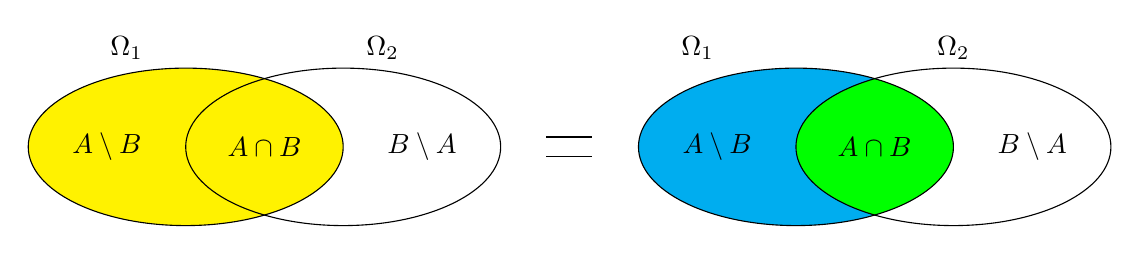
\begin{tikzpicture}[scale=0.5]
\begin{scope}
  \fill[yellow] (-3.5,1.5) ellipse (4 and 2);
\end{scope}
\begin{scope}
  \fill[cyan] (12,1.5) ellipse (4 and 2);
\end{scope}
\begin{scope}
  \clip (12,1.5) ellipse (4 and 2);
  \fill[green] (16,1.5) ellipse (4 and 2);
\end{scope}
%%
\draw (-3.5,1.5) ellipse (4 and 2);
\draw (0.5,1.5) ellipse (4 and 2);
\node at (-5.5,1.5) {$A\setminus B$};
\node at (-1.5,1.5) {$A\cap B$};
\node at (2.5,1.5) {$B\setminus A$};
\node at (-5,4) {$\Omega_1$};
\node at (1.5,4) {$\Omega_2$};
%% 
\draw (5.66,1.75) -- (6.82,1.75);
\draw (5.66,1.25) -- (6.82,1.25);
%%
\draw (12,1.5) ellipse (4 and 2);
\draw (16,1.5) ellipse (4 and 2);
\node at (10,1.5) {$A\setminus B$};
\node at (14,1.5) {$A\cap B$};
\node at (18,1.5) {$B\setminus A$};
\node at (9.5,4) {$\Omega_1$};
\node at (16,4) {$\Omega_2$};
\end{tikzpicture}
\end{center}

\br
As noted before, it suffices to know $P\big((-\infty,\lambda]\big)$ for all $\lambda \in \R$, and for this reason a new notation is introduced; \bse
P(\lambda) := P\big((-\infty,\lambda]\big).
\ese 
However, as they are written they appear to have different domains. We therefore give a new name to $P(\lambda)$; the \emph{resolution of the identity}\index{resolution of the identity}. 
\er

\subsection{Real and Complex Valued Borel Measures Induced by a PVM}

\bd 
For all $\psi,\varphi\in\cH$ we define the $\C$-valued measure 
\bi{rrCl}
\mu_{\psi,\varphi} \cl & \sigma(\cO_{\R}) & \to & \C\\
& \Omega  & \mapsto & \mu_{\psi,\varphi}(\Omega) := \braket{\psi}{P(\Omega)\varphi}.
\ei
\ed 

\bd 
For all $\psi\in\cH$ we define the $\R$-valued measure
\bse 
\mu_{\psi} := \mu_{\psi,\psi}
\ese 
\ed 

\bq that $\mu_{\psi}(\Omega)\in\R$. 
\bi{rCl}
\mu_{\psi}(\Omega) & = & \braket{\psi}{P(\Omega)\psi} \\
& = & \braket{P(\Omega)\psi}{\psi} \\
& = & \overline{\braket{\psi}{P(\Omega)\psi}} \\
& = & \overline{\mu_{\psi}(\Omega)},
\ei 
where we have used the fact that $P$ is self adjoint to go from the first to the second line. 
\eq

\subsection{Integration With Respect to a PVM}

We now wish to make sense of the operator $\int_{\R}fdP$ for measurable $f:\R\to\C$. We will build this up in three steps: 

\ben[label=(\roman*)]
\item For simple $f$, 
\item For bounded $f$, and 
\item For not necessarily bounded\footnote{Recall footnote 5 from lecture 2: to us the term `unbounded' means definitely \textit{not} bounded.} $f$. 
\een 

\br 
As we shall see, if $f$ is bounded (in the sense that there exists a $a\in\R$ such that $|f(x)|<a$ for all $x\in\R$) that the integral part of the operator will have nice properties. For example it will be linear in $f$, i.e. 
\bse 
\int_{\R}(\alpha f + g) dP = \alpha \int_{\R}fdP + \int_{\R}gdP,
\ese 
for $\alpha\in\C$. However, if $f$ is unbounded, domain issues will destroy the equality above. It is important to note, though, that it is exactly the latter case we need as 
\bi{rrCl}
f= i_{\R} \cl & \R & \hookrightarrow & \C\\
& x & \mapsto & x 
\ei 
in the Spectral theorem, which is clearly unbounded. 
\er 

\subsubsection*{A. \ Simple $f$}

Recall a simple function is a measurable function that takes a finite number of results in the target, i.e. if $f\cl\R\to\C$ then
\bse
f(\R) = \{f_1,...,f_N\} \ss \C
\ese 
for some $N\in\N$. This allows us to rewrite $f$ as
\bse 
f = \sum_{n=1}^N f_n \chi_{\Omega_n},
\ese 
where $\Omega_n := \preim_f(\{f_n\})$ and $\chi$ is the characteristic function.

\bd 
For simple $f:\R\to\C$ and PVM $P$ we define 
\bse
\int_{\R}fdP := \sum_{n=1}^Nf_nP(\Omega_n).
\ese 
\ed 

\bp 
For simple $f$, $\int_{\R}fdP$ is linear in $f$.
\ep 

\bq 
Let $S(\R,\C)$ denote the set of all simple functions $f:\R\to\C$. We can make this set into a $\C$-vector space by inheriting the addition and $s$-multiplication from $\C$, namely define 
\bse
(f+g)(x) := f(x) + g(x), \qquad (\alpha\cdot f)(x) := \alpha\cdot f(x),
\ese 
for all $f,g\in S(\R,\C)$, $\alpha\in\C$. 

Now consider the preimage part: As $f$ and $g$ are both simple it follows that 
\bse 
(f+g)(x) = f_n + g_n 
\ese 
for some $f_n,g_n\in\C$, so the preimage term becomes
\bi{rCl}
\preim_{f+g}\{f_n+g_n\} = \{x\} & = & \preim_{f}\{f_n\} \\
& = & \preim_{g}\{g_n\}.
\ei
It follows trivially, then, that 
\bse 
\int_{\R} (f+g)dP = \int_{\R}fdP + \int_{\R}gdP.
\ese 

A similar method gives the $\alpha\in\C$ condition of linearity. 
\eq 

\br 
\label{rmk:CharacteristicPVM}
Observe that $\chi_{\Omega}$ for any $\Omega\in\sigma(\cO_{\R})$ is simple (it only takes the values 0 or 1), and hence 
\bse
\int_{\R}\chi_{\Omega} dP = 1\cdot P(\Omega) + 0\cdot P(\sigma\setminus\Omega) = P(\Omega).
\ese 
\er 

\br
Observe also that for any $\psi,\varphi\in\cH$, 
\bi{rCl}
\braket{\psi}{\bigg(\int_{\R}fdP\bigg)\varphi} & = & \braket{\psi}{\sum_{n=1}^N f_n P(\Omega_n) \varphi} \\
& = & \sum_{n=1}^Nf_n \braket{\psi}{P(\Omega_n)\varphi} \\
& = & \sum_{n=1}^N f_n \mu_{\psi,\varphi}(\Omega_n) \\
& =: & \int_{\R} f d\mu_{\psi,\varphi},
\ei 
where \Cref{prp:MeasureIntegral} was used.
\er 

\bd 
For simple $f$ we can define the map 
\bi{rrCl}
\bigg(\int_{\R}dP\bigg) \cl & S(\R,\C) & \to & \cL(\cH) \\
& f & \mapsto & \int_{\R}fdP,
\ei 
which, if we equip $S(\R,\C)$ with the suppremum norm and $\cL(\cH)$ with its operator norm, has operator norm $\|\int_{\R}dP\| = 1$.
\ed 

\bq 
We have already shown that $\int_{\R}fdP \in\cL(\cH)$ (i.e. it is linear), so we just need to show the norm condition. First, let $f\in S(\R,\C)$ and $\psi\in\cH$, then
\bi{rCl}
\bigg{\|}\bigg(\int_{\R}fdP\bigg)\psi\bigg{\|}_{\cH}^2 & = & \braket{\bigg(\int_{\R}fdP\bigg)\psi}{\bigg(\int_{\R}fdP\bigg)\psi} \\
& = & \braket{\sum_{n=1}^Nf_nP(\Omega_n)\psi}{ \sum_{m=1}^Nf_m P(\Omega_m) \psi} \\
& = & \braket{\psi}{ \sum_{n,m=1}^N \overline{f_n} f_m P(\Omega_n) P(\Omega_m) \psi} \\
& = & \braket{\psi}{\sum_{n,m=1}^N \overline{f_n} f_m \delta_{nm} P(\Omega_m) \psi} \\
& = & \sum_{n=1}^N |f|^2 \braket{\psi}{P(\Omega_n)\psi} \\
& = & \sum_{n=1}^N |f|^2 \mu_{\psi}(\Omega_n) \\
& =: & \int_{\R} |f|^2 d\mu_{\psi} \\
\implies \bigg{\|}\bigg(\int_{\R}fdP\bigg)\psi\bigg{\|}_{\cH} & \leq & \|f\|_{\infty}\|\psi\|_{\cH},
\ei 
where we have used the definition of the norm in terms of the inner product, the fact that $P$ is self adjoint, the fact that $P(\Omega_n)P(\Omega_m) = \delta_{nm}$ for pairwise disjoint $\Omega_n/\Omega_m$, and \Cref{prp:NormLp} along with the fact that $\|f\|_{\infty} := \sup_{x\in\R}f(x)$. The equality in the last line can be assumed provided $f$ and $\psi$ are sufficiently chosen. 

Thus we have 
\bi{rCl}
\bigg{\|} \int_{\R}dP\bigg{\|} & := & \sup_{f\in S(\R,\C)}  \frac{\big{\|}\int_{\R}fdP\big{\|}_{\cL(\cH)}}{\|f\|_{\infty}} \\
& := & \sup_{f\in S(\R,\C)} \sup_{\psi\in\cH} \frac{\big{\|}\big(\int_{\R}fdP\big)\psi\big{\|}_{\cH}}{\|f\|_{\infty}\|\psi\|_{\cH}} \\
& = & 1.
\ei 
\eq 

\subsubsection*{B. \ Bounded Borel Functions}

\bd 
The set of all bounded, measurable functions is denoted 
\bse 
\cB(\R,\C) := \{f\cl\R\to\C \,|\, \text{measurable}, \|f\|_{\infty} <\infty\}.
\ese
\ed 

\bp 
The set $\cB$ can be made into a Banach space by defining the norm 
\bse 
\|f\|_{\cB} := \sup_{x\in\R} |f(x)|.
\ese 
\ep 

\bq 
We turn the set into a linear vector space in the usual manner; we inherit the addition and $s$-multiplication from $\C$. 

Now prove $\|f\|_{\cB}$ is a norm. Comparing to the definition given at the bottom of Page 9, for $f,g\in\cB(\R,\C)$ and $z\in\C$ we have 
\ben[label=(\roman*)]
\item Clearly $\|f\|_{\cB} \geq 0$.
\item 
\bi{rCl}
\|f\|_{\cB} & = &  0 \\ 
\eqv \sup_{x\in\R}|f(x)| & = & 0 \\
\eqv f(x) & = & 0 \qquad \forall x\in\R
\ei 
so $f=0$. 
\item 
\bi{rCl}
\|z\cdot f\|_{\cB} & := & \sup_{x\in\R}|z\cdot f(x)| \\
& = & |z|\sup_{x\in\R}|f(x)| \\
& =: & |Z|\cdot \|f\|_{\cB}.
\ei 
\item 
\bi{rCl}
\|f+g\|_{\cB} & := & \sup_{x\in\R} |(f+g)(x)| \\
& = & \sup_{x\in\R}|f(x)+g(x)| \\
& \leq &  \sup_{x\in\R}|f(x)|+ \sup_{x\in\R}|g(x)| \\
& =: & \|f\|_{\cB} + \|g\|_{\cB}.
\ei
\een

Now let $\{f_n\}_{n\in\N}$ be a Cauchy sequence in $\cB(\R,\C)$, that is: $\forall \epsilon>0, \exists N\in\N \cl \forall m,n\geq N$ we have 
\bse 
d(f_n,f_m) := \|f_n - f_m\|_{\cB} := \sup_{x\in\R} |f_n(x)-f_m(x)| < \epsilon.
\ese 

Now from the definition of the supremum we have 
\bse 
|f_n(x) - f_m(x)| \leq \|f-g\|_{\cB},
\ese 
so it follows that the sequence $\{f_n(x)\}_{n\in\N}$ is a Cauchy sequence in $\C$. But $\C$ is a complete metric space so we know that this Cauchy sequence converges in $\C$, i.e. 
\bse 
\lim_{n\to\infty} f_n(x) = z_x \in \C.
\ese 
We can thus define a point-wise limit $f$ of the sequence $\{f_n\}_{n\in\N}\ss \cB(\R,\C)$ as
\bse 
f(x) := \lim_{x\to\infty} f_n(x) = z_x
\ese 
for all $x\in\R$. Then, by equipping $\C$ and $\R$ with their respective Borel $\sigma$-algebras, \Cref{prp:MeasurablePointwiseLimit} tells us that $f$ is measurable. 

Finally from the fact that $\cB(\R,\C) \ss \cL(\R,\C)$, \Cref{thrm:BoundedLinearOperatorsBanach} tells us that $f$ is bounded and so $\cB(\R,\C)$ is a Banach space. 
\eq 

\bc
Observe that $S(\R,\C)$ is in-fact a dense, linear subspace of $\cB(\R,\C)$. Thus, the BLT theorem tells us that we have a unique extension of the operator 
\bse 
\bigg(\int_{\R}dP\bigg) \cl S(\R,\C) \to \cL(\cH)
\ese 
to the domain $\cB(\R,\C)$ with equal operator norm. That is, we have an operator 
\bse 
\widehat{\bigg(\int_{\R}dP\bigg)} \cl \cB(\R,\C) \to \cL(\cH)
\ese 
with $\big{\|}\widehat{\int_{\R}dP}\big{\|}=1$. 
\ec 

\bc 
By suitable definition we can turn the space $\cB(\R,\C)$ into an $C^*$-algebra and our operator then has the following properties 
\ben[label=(\roman*)]
\item \bse 
\int_{\R} 1 dP = \id_{\cH} 
\ese 
\item \bse 
\int_{\R}(f\cdot g)dP = \bigg(\int_{\R}fdP\bigg) \circ \bigg(\int_{\R}gdP\bigg)
\ese 
\item \bse 
\int_{\R}\overline{f}dP = \bigg(\int_{\R}fdP\bigg)^*
\ese
\een
These properties collectively make the operator a $C^*$-algebra homomorphism.
\ec 

\subsubsection*{C. \ General Borel Function}

We now want to allow for the case that $f$ is unbounded. We will write the following such that it reduces to the above when $f$ is bounded. 

\bd 
Let $f:\R\to\C$ be measurable, then we define the linear map 
\bse 
\bigg(\int_{\R} fdP\bigg) \cl \cD_{\int_{\R}fdP} \to \cH
\ese 
where 
\bse 
\cD_{\int_{\R}fdP} := \bigg{\{}\psi\in\cH \,\Big{|}\, \int_{\R}|f|^2 d\mu_{\psi} < \infty\bigg{\}} \se \cH,
\ese 
is a dense, linear subspace. The linear map is defined via 
\bse 
\bigg(\int_{\R}fdP\bigg)\psi := \lim_{n\to\infty} \bigg[\bigg(\int_{\R}f_ndP\bigg)\psi\bigg],
\ese
where the sequence $\{f_n\}_{n\in\N}\se \cB(\R,\C)$ defined by 
\bse 
f_n := \chi_{\{x\in\R|f(x)<n\}} f.
\ese 
\ed 

\br 
Note that the map above includes the $f$, it is not just the integral defined in the previous section. Note also for the case when $f\in\cB(\R,\C)$ we just recover the case above and we have $\cD_{\int_{\R}fdP}=\cH$ (i.e. we have $\cL(\cH)$). Otherwise it is a proper  subset.
\er 

\br 
The literature often introduces the notation 
\bse 
\cD_f := \cD_{\int_{\R}fdP},
\ese 
however this could lead one to think of the domain of $f$ itself, which here is $\R$. We will avoid this notation.
\er 

\br
The sequence $\{f_n\}_{n\in\N}$ can be thought of as `chopping' $f$ into bounded parts. 

\begin{center}
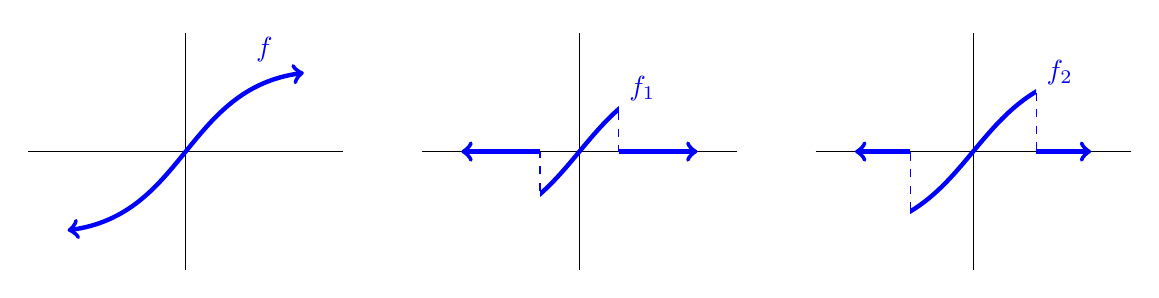
\begin{tikzpicture}
\draw (-10,0) -- (-6,0);
\draw (-8,-1.5) -- (-8,1.5);
\draw[blue, ultra thick, <->] (-9.5,-1) .. controls (-8, -0.8) and (-8,0.8) .. (-6.5,1);
\node at (-7,1.3) {\textcolor{blue}{$f$}};
%%
\draw (-5,0) -- (-1,0);
\draw (-3,-1.5) -- (-3,1.5);
\begin{scope}
  \clip (-3.5, 1.5) rectangle (-2.5,-1.5);
  \draw[blue, ultra thick] (-4.5,-1) .. controls (-3, -0.8) and (-3,0.8) .. (-1.5,1);
\end{scope}
\draw[blue, dashed] (-3.5,-0.5) -- (-3.5,0);
\draw[blue, dashed] (-2.5,0.5) -- (-2.5,0);
\draw[blue, ultra thick, ->]  (-3.5,0) -- (-4.5,0); 
\draw[blue, ultra thick, ->] (-2.5,0) -- (-1.5,0);
\node at (-2.2,0.8) {\textcolor{blue}{$f_1$}};
%% 
\draw (0,0) -- (4,0);
\draw (2,-1.5) -- (2,1.5);
\begin{scope}
  \clip (1.2, 1.5) rectangle (2.8,-1.5);
  \draw[blue, ultra thick] (0.5,-1) .. controls (2, -0.8) and (2,0.8) .. (3.5,1);
\end{scope}
\draw[blue, dashed] (1.2,-0.75) -- (1.2,0);
\draw[blue, dashed] (2.8,0.75) -- (2.8,0);
\draw[blue, ultra thick, ->] (1.2,0) -- (0.5,0);
\draw[blue, ultra thick, ->] (2.8,0) -- (3.5,0);
\node at (3.1,1) {\textcolor{blue}{$f_2$}};
\end{tikzpicture}
\end{center}
\er 

\bl 
The sequence $\{f_n\}_{n\in\N}$ is Cauchy in $L^2(\R)$. This in tern implies that the sequence $\{(\int_{\R}f_ndP)\psi\}_{n\in\N}$ is Cauchy in $\cH$, which is required for the limit in the definition to make sense, i.e. the result lies in $\cH$.
\el 

For this general case of a measurable $f$ we have:
\ben[label=(\roman*)]
\item As before
\bse 
\int_{\R}\overline{f}dP = \bigg(\int_{\R}fdP\bigg)^*.
\ese 
\item For $\alpha\in\C$ and $f,g$ measurable,
\bse 
\bigg(\alpha \int_{\R}fdP + \int_{\R}gdP \bigg) \se \int_{\R}(\alpha f + g)dP,
\ese 
where the equality holds only for bounded $f$. As explained earlier, the inequality arises due to domain issues. We can now see this more explicitly from the definition of $\cD_{\int_{\R}fdP}$; just because $f$ and $g$ are both measurable, it does not mean that their respective map domains will coincide. However, the domain for the LHS is $\cD_{\int_{\R}(|\alpha f| + |g|)dP}$.
\item \bse 
\bigg(\int_{\R}fdP\bigg)\circ \bigg(\int_{\R}gdP\bigg) \se \int_{\R}(f\cdot g)dP,
\ese 
again where the equality holds only when $f$ and $g$ are bounded.
\een

\subsection{The Inverse Spectral Theorem}

We are now in a place where we can understand the inverse spectral theorem. 

\bd 
Given a PVM, $P$, we can construct a self adjoint operator $A_P$ as 
\bse 
A_P := \int_{\R} \id_{\R} dP,
\ese 
where $\id_{\R}\cl \R\hookrightarrow \C$ is the inclusion map. 
\ed 

\bq 
\bi{rCl}
(A_P)^* & = & \int_{\R} \overline{\id_{\R}} dP \\
& = & \int_{\R} \id_{\R} dP \\
& = & A_P,
\ei 
so $A_P$ is self adjoint. 
\eq 